\begin{appendices}
\chapter{Chapter \ref{chp:4} supplementary material} \label{app:chap4}

\section{Proof of convergence of the parametric change-point detection model}\label{app:chap4:1}

\section{Newton-Raphson initialization experiments}\label{app:chap4:2}

\section{Convergence of \texorpdfstring{$\hat\sigma$}{s}}\label{app:chap4:3}

The experimental protocol is the following. We simulated $N = 100$ samples of size $n = 320$ of left censored Weibull realisations. 3 change points are present in the samples at position $80$, $160$ and $240$. The associated parameters for each segment are $(1,1/100,1/100,1)$. Four scenarios are proposed where the $\sigma^*$ and the censoring rate $\alpha$ varies. We test all configuration possible for $\sigma^* = (0.4,0.8)$ and $\alpha = (25\%,75\%)$. All the results are presented in Figures \ref{fig:sim:sigma1} and \ref{fig:sim:sigma2}.     

\begin{figure}[ht]
    \centering
    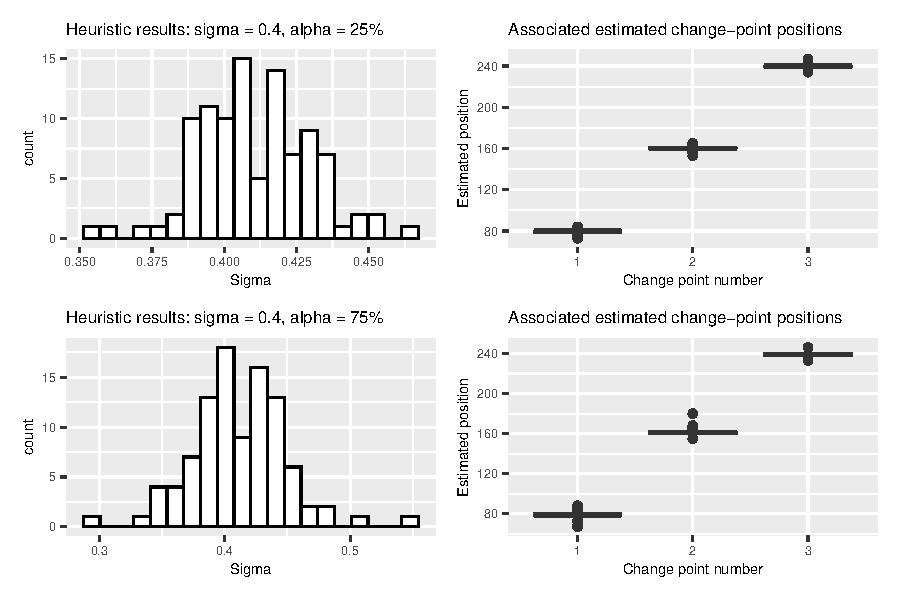
\includegraphics{figs/App/SIM_CHAP5_1.pdf}
    \caption{Scenarios with $\sigma = 0.4$.}
    \label{fig:sim:sigma1}
\end{figure}

\begin{figure}[ht]
    \centering
    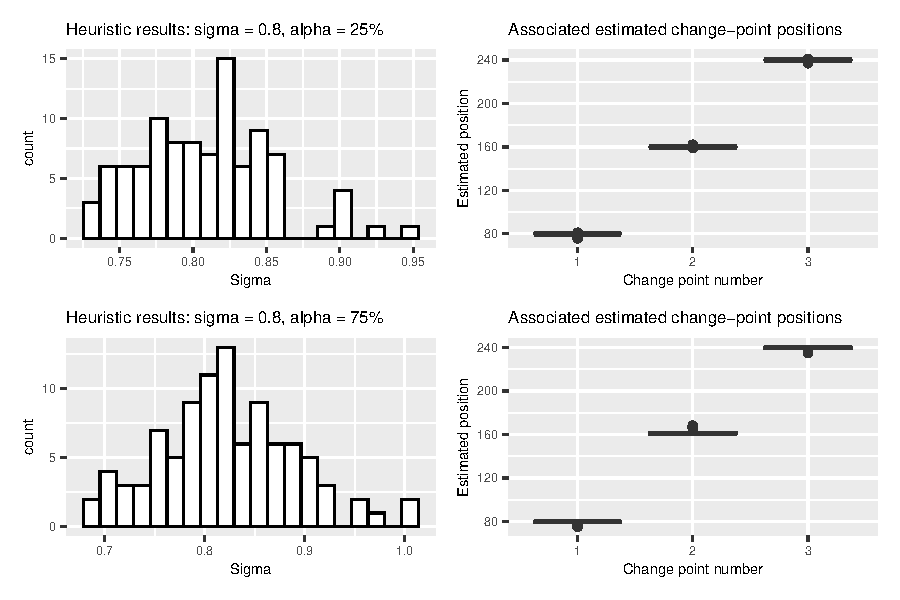
\includegraphics{figs/App/SIM_CHAP5_2.pdf}
    \caption{Scenarios with $\sigma = 0.8$.}
    \label{fig:sim:sigma2}
\end{figure}

For each of these samples, we use the heuristic proposed in \ref{subsection:pelt}. The penalty grid was defined by $Q = 5$ values set to $[\beta_0 = \frac{\ln n}{10},\dots,\beta_{q},\dots,\beta_{Q} = 5\ln n]$ with the $\beta_q$ being equidistant. We allowed this important range in the penalties to ensure enough distinct points for the elbow heuristic. The only PELT parameter that wasn't set as in Chapter \ref{chp:4} was the minimal segment size. It was set to 25. The choice was motivated by the computational time of the simulations, even though we have seen that the estimation of the detection capacity of our method is lower with this minimal segment size. In the procedure, the first iteration $\widehat{\sigma}_0$ is computed with the \texttt{fitdistr} R package \cite{delignette2015}. In the second step of the heuristic, minimizing \ref{new:lk} with respect to $\sigma$ is done using \cite{Byrd1995} which allows for a box constraint for the parameter value $\sigma$ (lower and upper bounds). This interval was set to $[0,1]$. This explains that the estimated values are all inferior to 1 in Figure \ref{fig:sim:sigma2}. We defined a stopping criterion to the heuristic depending on the $\widehat{\sigma}$ values that consists in stopping when the upgrade of the new $\widehat{\sigma}$ is not superior to $10^-3$.


\chapter{Chapter \ref{chp:5} supplementary material}\label{app:chap5}

\section{Clustering algorithms}\label{app:clustalgo:chap5}

We keep the same notations than in \ref{subsection:pelt}. We introduce the following new notations : 
\begin{itemize}
    \item $C_m^p$ the $m$-th cluster located in component $p$.
    \item $M_p$ the number of clusters in component $\mathcal{K}_p$.
    \item $\displaystyle Q(\mathcal{K}_p,C_m^p) = \frac{1}{\lvert C_m^p\rvert}\sum_{v_i,v_j \in C_m^p}d_{ij}^2$ the inertia of cluster $C^p_m$.
    \item $\displaystyle R_p(M_p) = \min_{(C_m^p)_{m=1}^{M_p}}\sum_{m = 1}^{M_p}Q(\mathcal{K}_p,C_m^p)$ the best partition (in the sense of minimal inertia) of component $p$ into $M_p$ clusters. 
    \item $\displaystyle S(l,m) = \min_{(M_p)_{p=1}^l \text{ such that } \sum_{p=1}^l M_p = m}\sum_{p=1}^lR_p(M_p)$ which is the best partition of the $l$ first components into a total number of $m$ clusters.
\end{itemize}

$R_p(m)$ can be computed with Ward hierarchical clustering technique. In the case of this work we used the \texttt{R} package \texttt{hclust}. With these notations, we can write the two developed methods as follows: 

\begin{algorithm}[ht]
\caption{Clustering with greedy method:}\label{algo:greed}
\begin{algorithmic}

\State \textbf{input} : the station graph $G=(V,E)$, the known partition into non connex components $(\mathcal{K_1},\dots,\mathcal{K}_P)$, a total number of clusters $M$ \\
  
\State \textbf{initialisation} : Compute $R_p(1)$ for all $p \in [1,\dots,P]$ using \texttt{hclust}, set $M_{opt} = (1,\dots,1)$ vector of size $P$  \\

\For{$m = 1$ to $M-P$}
  \State $\textit{score}\gets(0,\dots,0)$ vector of size $P$
  \For{$p = 1$ to $P$}
  \State $M_{opt}(p) \gets M_{opt}(p) + 1$
  \State $\textit{score}(p) \gets \sum_{p=1}^P R_p(M_{opt}(p))$
  \State $M_{opt}(p) \gets M_{opt}(p) - 1$
  \EndFor
  \State $\textit{pos} \gets which.min(\textit{score})$
  \State $M_{opt}(pos) \gets M_{opt}(pos)+1$
\EndFor
\For{$p=1$ to $P$}
\State built the optimal partition of $\mathcal{K}_p$ with $M_{opt}(p)$ clusters using \texttt{hclust}.
\EndFor

\end{algorithmic}
\end{algorithm} 

\begin{algorithm}[ht]
\caption{Clustering by dynamic programming:}\label{algo:dyn}
\begin{algorithmic}

\State \textbf{input} : the station graph $G=(V,E)$, the known partition into non connex components $(\mathcal{K_1}$, a total number of clusters $M$ \\
    
 \For{$p=1$ to $P$} : 
 \State Use \texttt{hclust} to compute $R_p(m)$ for all $m \in \{1,\dots,M-P+1\}$
 \EndFor 
 \For{$m=1$ to $M-P+1$} : 
 \State $S(1,m) \gets R_1(m)$ 
 \EndFor 
 \For{$l = 2$ to $P$} : 
  \For{$m = l$ to $M$} : 
     \State $W(l,m) \gets 1$ 
     \State $S(l,m) \gets S(l-1,m-1)+R_l(1)$
   \For{$u = 1$ to $m-l+1$}
   \If{$S(l-1,m-u)+R_l(u) < S(l,m)$}
     \State $W(l,m) \gets u$
     \State $S(l,m) \gets S(l-1,m-u)+R_l(u)$
   \EndIf
   \EndFor
 \EndFor 
 \EndFor 
 \State $M_{opt} \gets (\text{NA},\dots,\text{NA})$
 \State $P_{opt}(P) \gets W(P,M)$
 \State $\textit{left} \gets M-W(P,M)$
 \For{$p = P-1$ to $1$}
 \State $P_{opt}(p) \gets W(p,\textit{left})$
 \State $\textit{left} \gets \textit{left}-W(p,\textit{left})$
 \EndFor
 \For{$p = 1$ to $P$}
 \State built the optimal partition of $\mathcal{K}_p$ with $P_{opt}(p)$ clusters using \texttt{hclust}
 \EndFor 
\end{algorithmic}
\end{algorithm} 

\clearpage

\section{Modified empirical Wasserstein distance}\label{appendix:wasserstein}

The Wasserstein distance was chosen over the Kolmogorov-Smirnov or the Jensen-Shannon metric. It has the advantage of integrating in the distance calculation both the differences between the probabilities of observing different values but also the distances between those values. This is a critical point which is illustrated on a simple simulated example provided by Figure \ref{fig:ex_dist}. We show here three monitoring stations that have quite different behaviors. Those different behaviors are obvious both on in the temporal representation and in the histograms. However, the Kolmogorov-Smirnov distance between stations 1 and 3 is equal to the Kolmogorov-Smirnov distance between stations 1 and 2. This distance cannot capture the fact that station 2 recorded higher concentration values than station 3. On the contrary, the Wasserstein distance between stations 1 and 3 is smaller than the Wasserstein distance between stations 1 and 2. 

Computing information theoretic distances/dissimilarities such as the Jensen-Shannon divergence requires estimating densities for the distributions observed at the stations. As noted earlier, few concentration records (and even fewer quantified ones) are available at the level of a station and within a time period. Therefore, density estimations based on such a small number of observations are unreliable.

\begin{figure}[H]
    \centering
    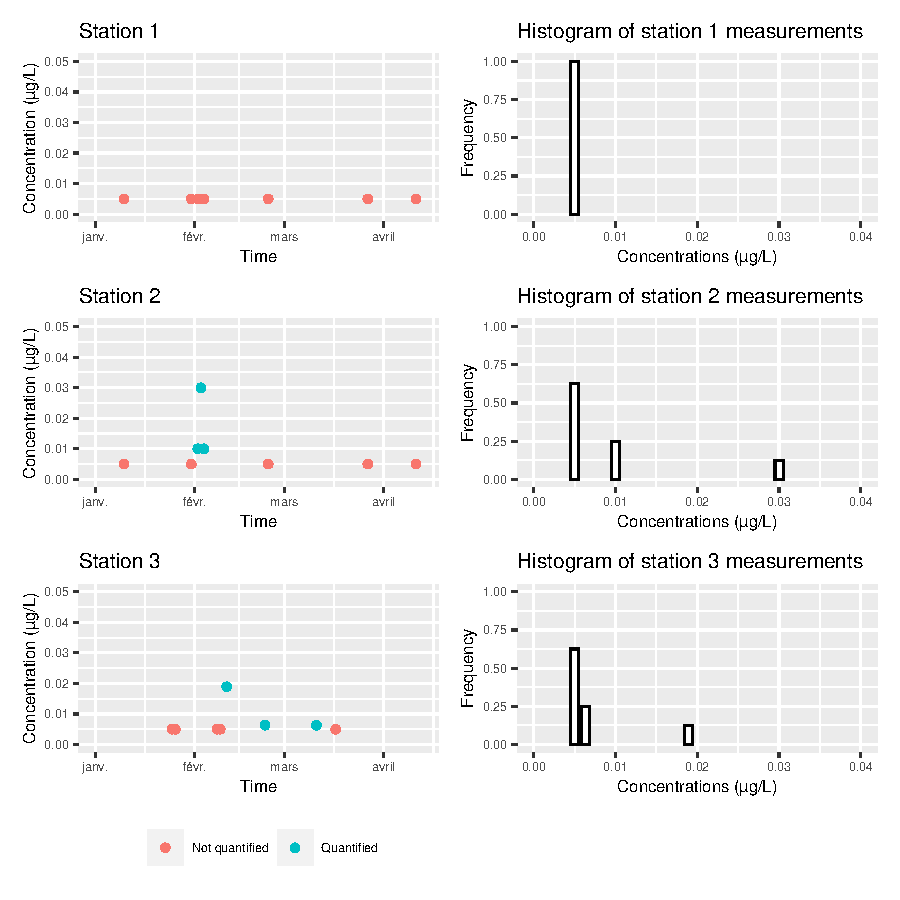
\includegraphics{figs/App/Simu_ex.pdf}
    \caption{Example of three stations data. The data were simulated.}
    \label{fig:ex_dist}
\end{figure}

The empirical 1-d Wasserstein distance used in our work is slightly adapted for left censored values. Given two samples $\bm{x}=(x_1,\dots,x_n)$ and $\bm{y}=(y_1,\dots,y_m)$ of sizes $n$ and $m$ with respective empirical c.d.f. $F_n$ and $G_m$, the 1-d empirical distance writes:
$$W_1(F_n,G_n) = \int_{\mathbbm{R}}\lvert F_n(x)-G_m(x) \rvert\mathrm{d}x$$
In the case of left censored observations, the empirical c.d.f. the first non zero value is the censoring threshold. If we use the classical empirical c.d.f., it does not take into account that the potential real values of censored samples is potentially lower than this threshold. In particular, if both samples $\bm{x}$ and $\bm{y}$ are fully censored at respective thresholds $a_1$ and $a_2$, the Wasserstein distance equals $\lvert a_1-a_2 \rvert$. We would like this quantity to be the smallest possible since none of the samples has any quantified values. Since the samples size for a single station is usually very small, a reasonable assumption is to suppose that the real values under the censoring threshold are uniformly distributed. Figure \ref{fig:mod_dist} illustrates the changes it implies on the empirical c.d.f.. In the previous example of $\bm{x}$ and $\bm{y}$, the adapted empirical distance gives $\lvert a_1-a_2\rvert/2$.    

\begin{figure}[H]
    \centering
    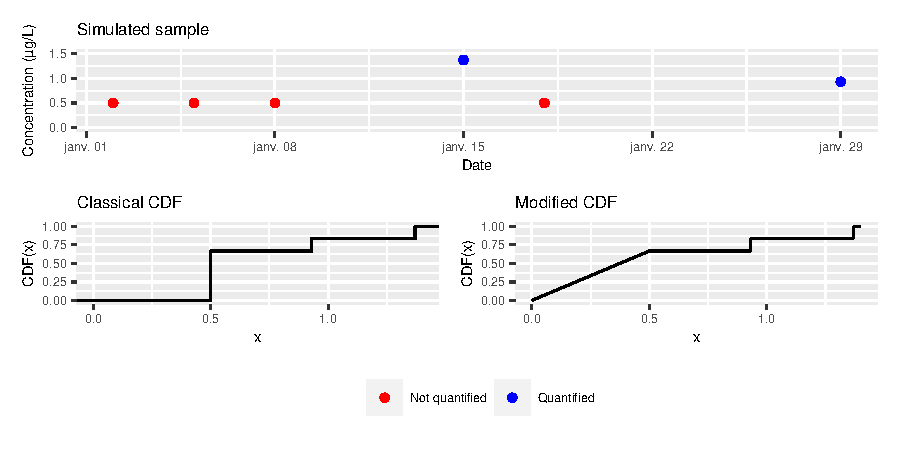
\includegraphics{figs/App/Wass_ew.pdf}
    \caption{Example of modified c.d.f. for the Wasserstein distance.}
    \label{fig:mod_dist}
\end{figure}

\section{Supplementary Figures}

\subsection{Regional map of crops}\label{section:crops}
The regional map of crops provided in Figure \ref{fig:crops} have been produced using data from the \emph{registre parcellaire graphique} produced by the IGN \cite{IGN:RPG}.

\begin{figure}[H]
    \centering
    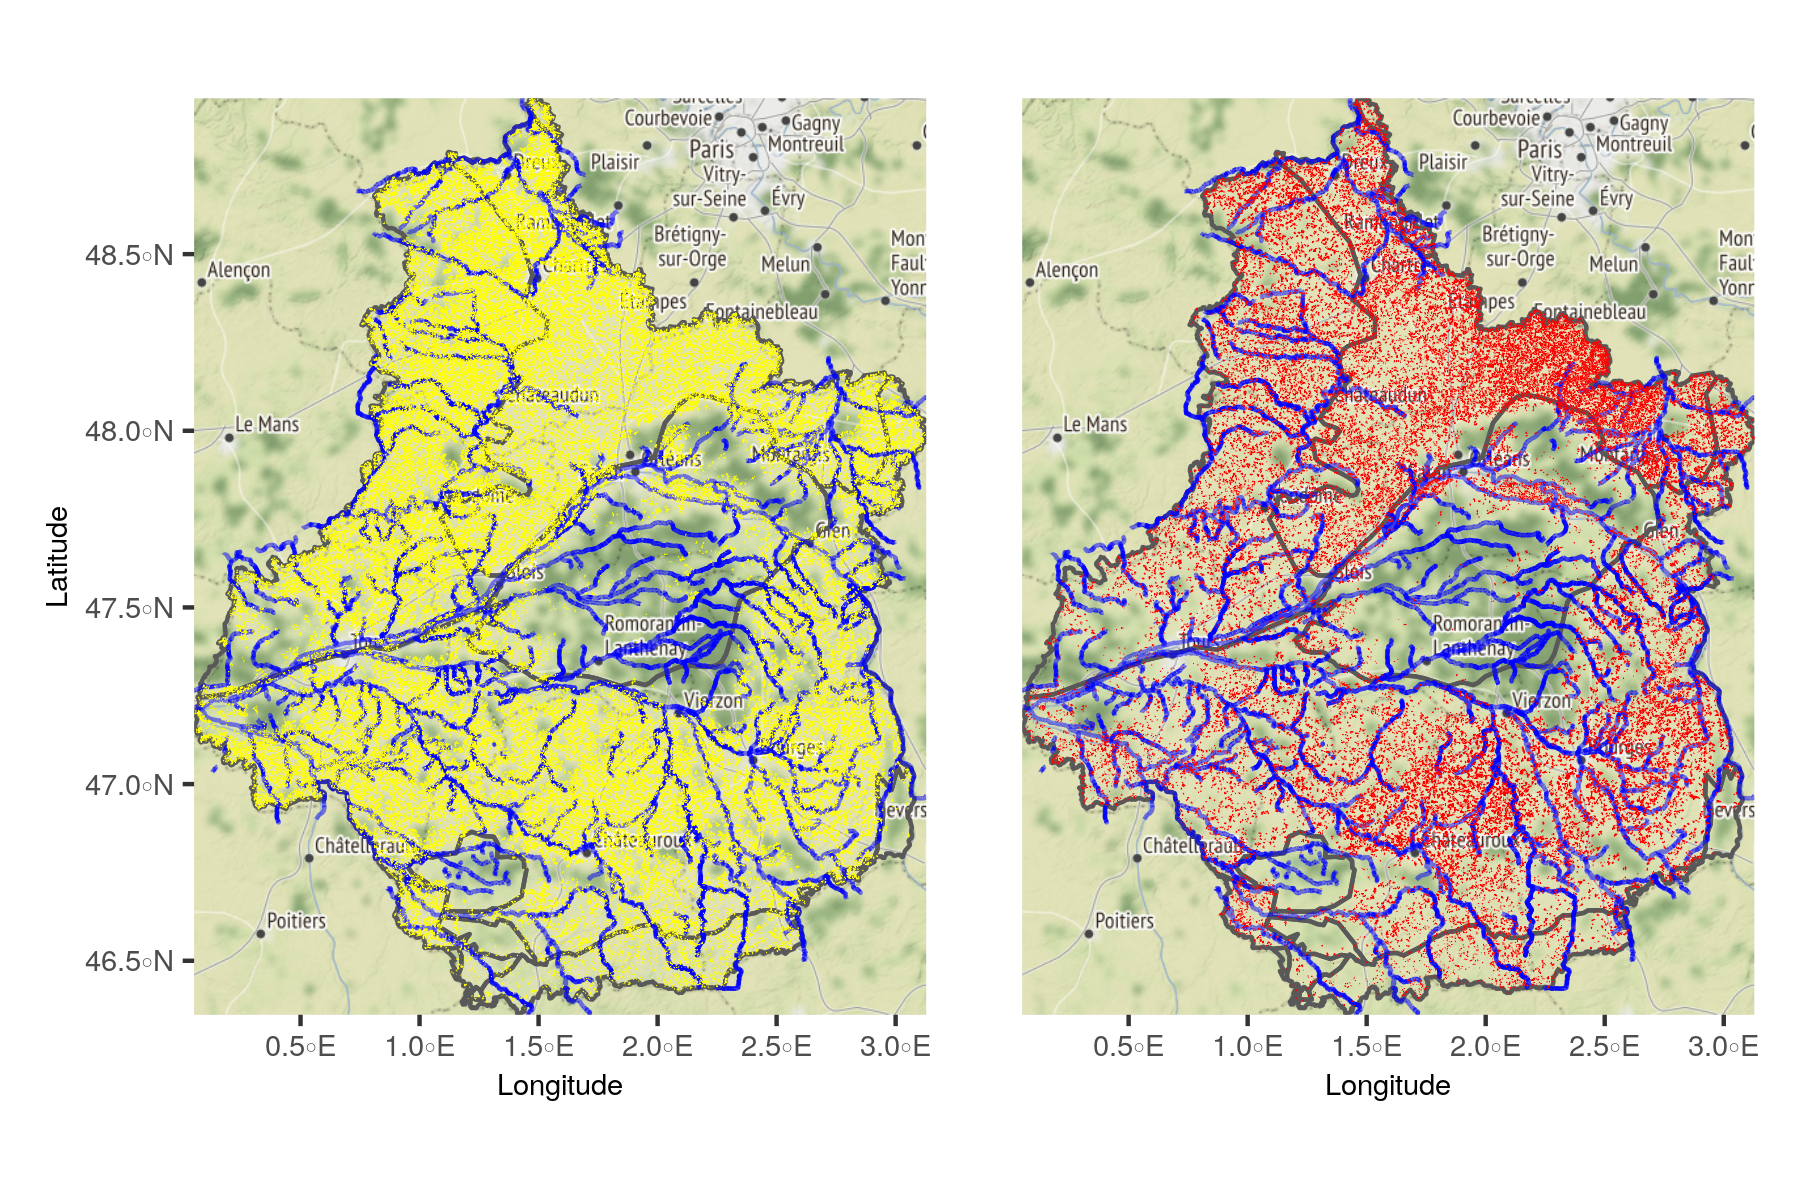
\includegraphics{figs/App/Occ_soil.png}
    \caption{Wheat (in yellow) and barley (in red) crops location in Centre-Val de Loire}
    \label{fig:crops}
\end{figure} 

\subsection{Prosulfocarb sales}\label{section:sale}

Prosulfocarb sales figures used to build Figure \ref{fig:sale} are made available by the \emph{Système d'information sur l'eau} \cite{BNVD}.

\begin{figure}[H]
  \centering
  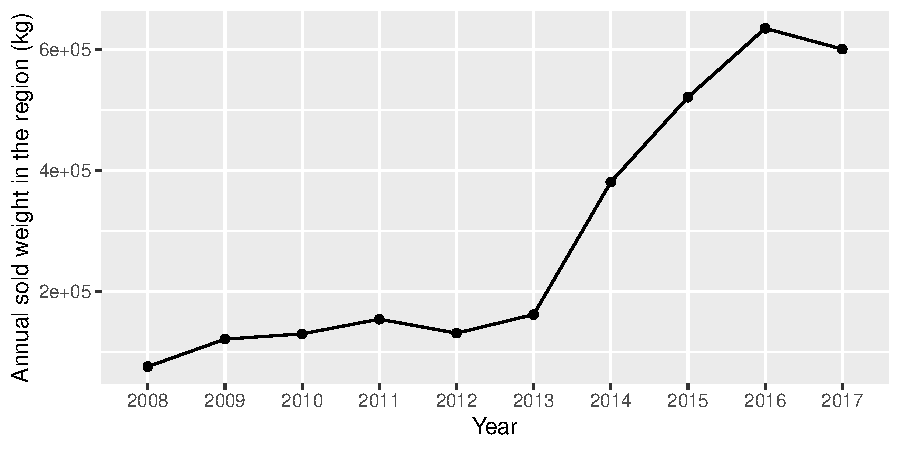
\includegraphics[]{figs/App/Sales_pro.pdf}
  \caption{Prosulfocarb sales between 2008 and 2017 in the Centre-Val de Loire region}
  \label{fig:sale}
\end{figure}

\subsection{All elbow methods figures}\label{section:elb}

\begin{figure}[H]
  \centering
  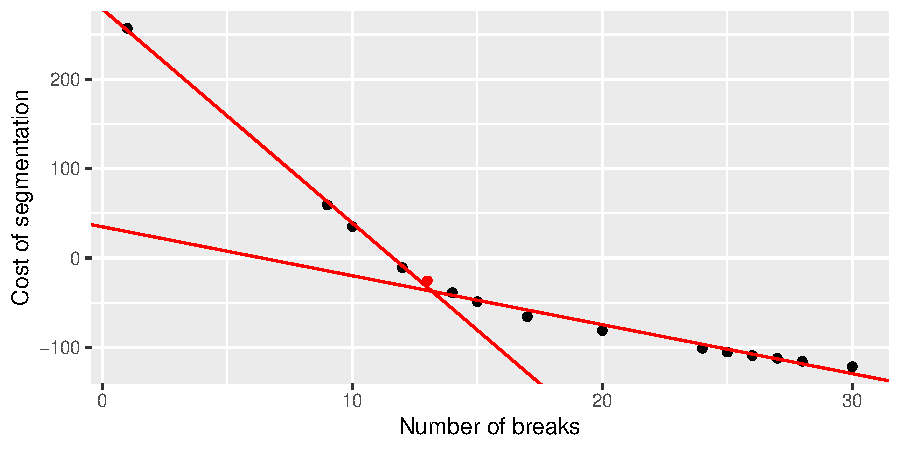
\includegraphics[]{figs/App/Elbow_seg.pdf}
  \caption{Elbow method selecting the optimal segmentation of the full signal $\overline{\mathcal{D}}$.}
  \label{fig:elb_seg}
\end{figure}

\begin{figure}[H]
  \centering
  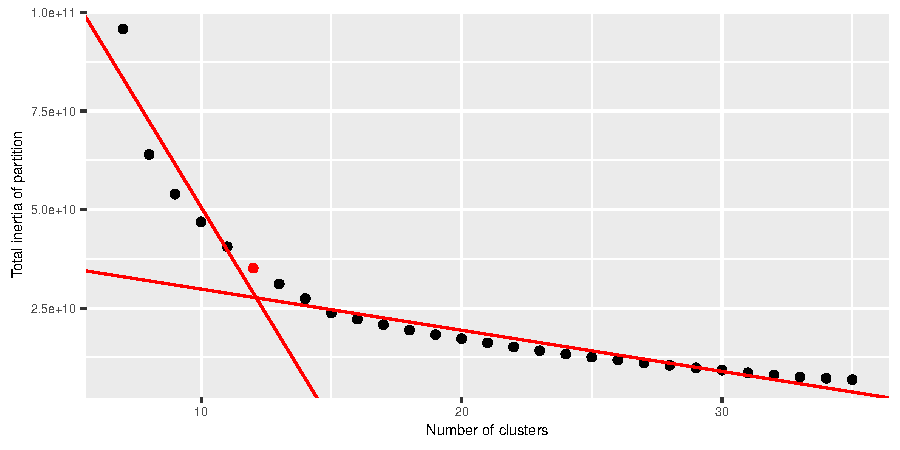
\includegraphics[]{figs/Chap5/Elb_clust.pdf}
  \caption{Elbow method for the spatial clustering.}
  \label{fig:elb:clust}
\end{figure}

\chapter{Chapter \ref{chp:6} supplementary material} \label{app:chap6}


\includepdf[pages=-, pagecommand={}]{8-Appendix/notice.pdf}

\end{appendices}